The data consists of 10000 samples and contains information on the item's color, the price, it's size and if it was returned by the customer or not. Additionally the data set encompasses information on the customers such as a unique identifier and the dates on which the item in question was ordered and delivered. With this information it is possible to retrieve the information on a complete order. In the following analysis an order is considered to be a collection of item orders that were placed by the same customer, on the same order date.

\begin{figure}
\centering
\caption{Conditional Probabilities of orders containing a returned item}
\label{exploratory}
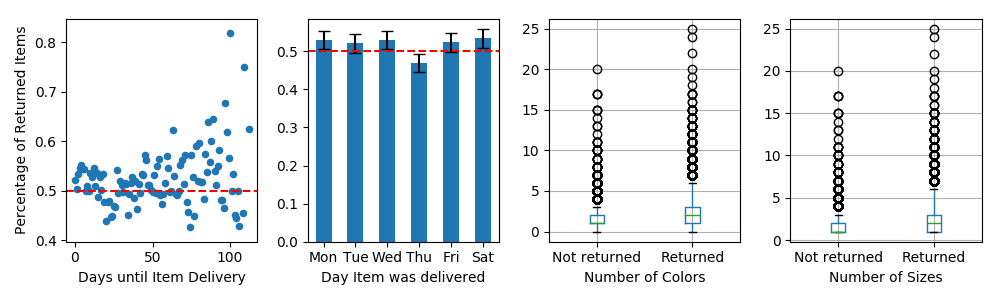
\includegraphics[scale=0.45]{../eda/exploratory.png}
\end{figure}

Figure \ref{exploratory} summarizes the initial findings through graphical evaluations of the data. It is apparent that a higher waiting time, i.e. the number of days that passes between ordering the item and it being delivered increases the likelihood of an item being returned. Additionally, it seems that items that are delivered on a Thursday on average get returned less. This difference is significant compared to all other days of the week, however the magnitude of this discrepancy is not substantial. Furthermore, the number of different sizes and the number of distinct colors in one order seem to differ slightly accross orders that contained a returned item compared to those who did not. Orders that were returned were both on average as well as in their 3rd quartile larger, and consisted of a broader array of colors. Nevertheless, in their lower end both distributions are virtually indistinguishable. This means that while there is a signal in the raw data it first needs to undergo a refining process before it can be used as a feature with a consequential predictive capacity. 

